%Correct the file name.
%X: book number
%Y: part number
%ZZZ: page number in three digits. So page 3 would be 003.

\documentclass[11pt]{amsbook}

\usepackage{../HBSuerDemir}	% ------------------------


\begin{document}

% ++++++++++++++++++++++++++++++++++++++
\hPage{feyzioglu-069}
% ++++++++++++++++++++++++++++++++++++++

\begin{center}

    $(a,(b+d)+f)\stackrel{?}{=}(a,b+(d+f))$

\end{center}

Yes, this is true since + is an associative operation on $\mathbb{Z}$. Hence $\Delta$, is\par
associative.

\begin{center}

    (iii) Is there an element in $\mathbb{Z}x\mathbb{Z},(a_{0},b_{0})$ say, such that\\
    $(a,b)\Delta(a_{0},b_{0})=(a,b)$ for all $(a,b)\in \mathbb{Z}x\mathbb{Z}? $

\end{center}

Well, this is true if and only if $(a,b+b_{0})=(a,b)$, which is equivalent to\par
$b_{0}=0$. There is no condition on $a_{0}$. For example,\\

\begin{center}

    $(a,b)\Delta(0,0)=(a,b+0)=(a,b)$\\
    $(a,b)\Delta(1,0)=(a,b+0)=(a,b)$

\end{center}

for all $(a,b)\in\mathbb{Z}x\mathbb{Z}$, so (0,0) and (1,0) are right identities. In fact, any\par
$(n,0)\in\mathbb{Z}x\mathbb{Z}$ is a right identity.\par
From Lemma 7.3, we know that a group has one and only one right\par
identity. so $\mathbb{Z}x\mathbb{Z}$ is not a group under $\Delta$. On the other hand, with\par
respect to (0,0) for example (in fact, with respect to any right identity),\par
each element (a,b) of $\mathbb{Z}x\mathbb{Z}$ has a left inverse (0,-b):

\begin{center}

    $(0,-b)\Delta(a,b)=(0,-b+b)=(0,0)$

\end{center}

(with respect to (n,O), a left inverse of (a,b) is (n,-b)).\par

So $(\mathbb{Z}x\mathbb{Z},\Delta)$ is a system in which a right identity exists, plus a left\par
inverse of each element; nevertheless, it fails to be a group. Likewise,\par
fulfilling the existence of a left identity and right inverses is not enough\par
for building a group.\par

We could define a group by including the claims of Lemma 7.3 directly\par
into the definition. Then we would have\par

\begin{center}

    (iii) there is a unique $e\in\mathbb{G}$ such that\\
    $a\circ e=e\circ a=a$ for all $a\in\mathbb{G}$

\end{center}

and

\begin{center}

    (iv) for all $a\in\mathbb{G}$, there is a unique $a^{-1}\in\mathbb{G}$ such that\\
    $a\circ a^{-1}=e=a^{-1} \circ a$

\end{center}

in place of (iii) and (iv) of definition 7.2. Some textbooks define groups\par
in this way. This would save us from the trouble of proving Lemma 7.3.\par
Why, then, did we not use this definition? Because we do not want to\par
do unnecessary work. If we defined groups by (iii)' and (iv)' instead of\par
(iii) and (iv), then, each time when we wanted to show that a set $\mathbb{G}$\par
builds a group under a binary operation $\circ$ on $\mathbb{G}$, we had to check

\begin{center}

    \begin{enumerate}
        \item that there is an $e\in\mathbb{G}$ such that $a\circ e=a$ for all $a\in\mathbb{G}$. 
        \item that this $e$ is also such that $e\circ a=a$ for all $a\in\mathbb{G}$.
    \end{enumerate}

\end{center}



% =======================================================
\end{document}  

%==== templates ====

%==== environments ====

%\begin{figure}[htb]
%	\centering
%	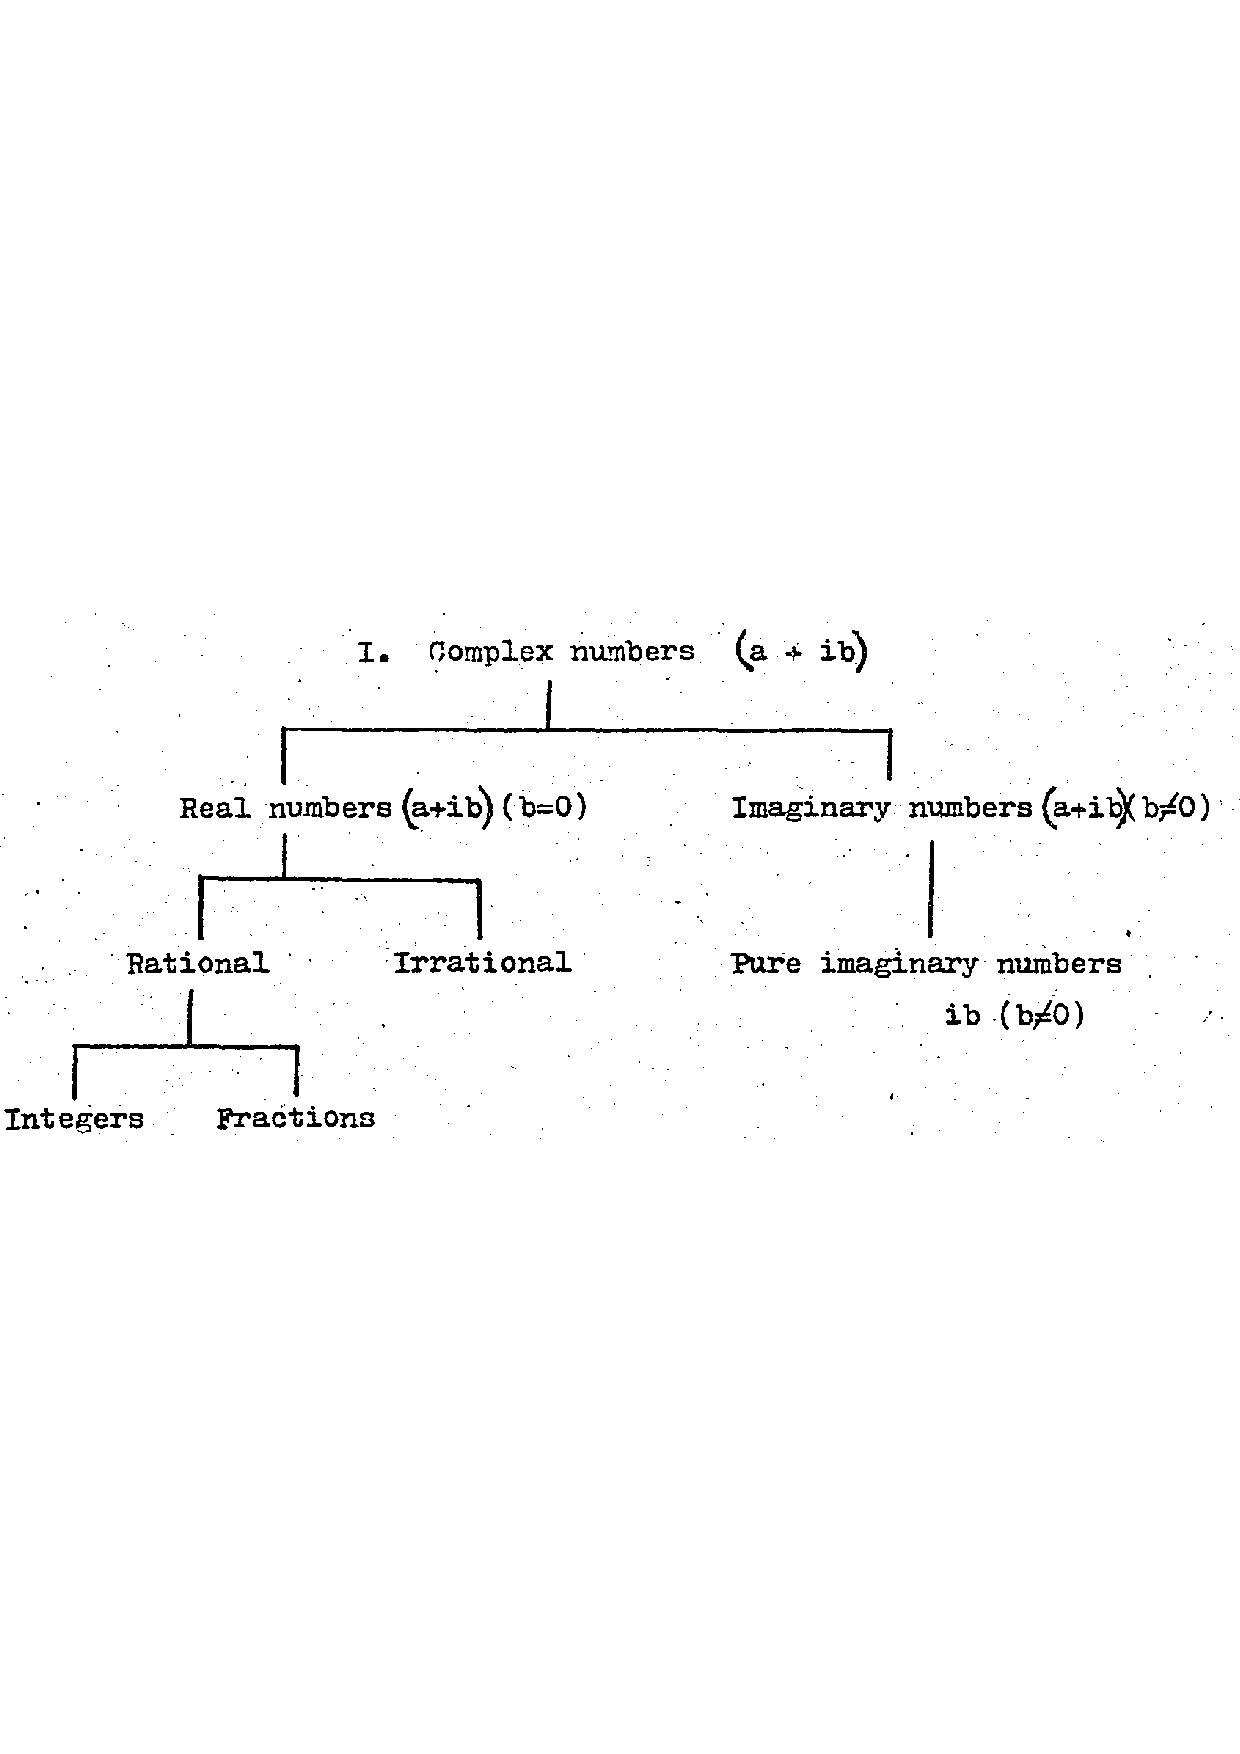
\includegraphics[width=0.9\textwidth]{images/SD-1-1p15A}
%	\caption{Classification of complex numbers}
%	\label{fig:classificationOfComplexNumbersA}
%\end{figure}

%\begin{center}
%\begin{tabular}{cc}
%\end{tabular}
%\end{center}

%\begin{exmp}
%\begin{hSolution}
%\end{hSolution}
%\end{exmp}

%\begin{hEnumerateAlpha}
%\end{hEnumerateAlpha}

%\begin{hEnumerateRoman}
%\end{hEnumerateRoman}

%$
%\begin{bmatrix}
%\end{bmatrix}
%$

%\frac{aaaa}{bbb}
%\frac{a_{n}}{b_{n}}
%\left( aaaa \right)
%\Longrightarrow

%\begin{multicols}{2}
%	bb
%\columnbreak
%	aa
%\end{multicols}
